\chapter{Gestion de projet}
\minitoc

\section{Gestion de projet}
%Explication et distribution des roles scrum, vision du projet (objectifs, jalons, utilisateurs visés) et mise en place du backlog, estimations des points.

Le projet s'organise autour de la méthode agile Scrum, méthode qui nous a permis de maîtriser notre production et de la planifier. Ce projet a été réalisé en groupe avec une durée fixe à respecter et des objectifs clairs exprimés en début de projet (confère cahier des charges).

Afin de piloter au mieux le projet nous avons utilisé l'outil Youkan, un outils nous permettant de modéliser tout le processus projet. Cet outil nous a permis d'avoir une bonne traçabilité favorisant ainsi la collaboration entre les différents membres de l'équipe.
De part les différentes fonctionnalités offertes par YouKan, nous avons pu planifier et suivre les différentes étapes de notre projet et modéliser les exigences du client en gérant toute demande de modification.

La méthode Scrum nous a permis d'établir les estimations sur la difficulté et la durée des différentes tâches à réaliser. Pour cela, nous avons mis en place un backlog, nous avons listé les différentes tâches que nous avions à effectuer, et pour chacune d'entre elle nous avons à l'aide d'un système de point, pondéré la tâche en fonction de sa difficulté. 

Le projet a été découpé en 3 sprints, un sprint équivalent à une période de 21 jours. C'est donc un processus itératif qui a été utilisé tout au long de la réalisation du projet. Le premier sprint nous a permit d'évaluer les valeurs réelles de nos pondérations, c'est à dire, à combien de jour réel correspondait une pondération. Ainsi donc, nous avons pu avoir des estimations précise du temps nécessaire pour réaliser une tâche en fonction des compétences et de la cadence de travail de chacun des membres du groupe. 
De plus, Youkan dispose d'un Task Board faisant office de tableau virtuel sur lequel nous pouvons coller des post-it, post-it que nous pouvons coller dans une des quatres rubriques suivantes : Todo, In progress, Test et Done. Ainsi donc, l'ensemble de l'équipe peut se servir de se tableau pour suivre avec précision l'avancée du projet.

Afin de manager l'équipe, un responsable de projet nommé Scrum Master a été désigné, son rôle a été de s'assurer du bon déroulement du projet ainsi que de l'application de la méthode Scrum. Il a donc ainsi veillé à bien communiquer la vision et les objectifs du projet à l'équipe. Pour cela, c'est lui qui été chargé d'échanger avec le client et de restituer lors de réunion organisés les différentes attentes du client ainsi que les différents objectifs à atteindre durant le Sprint. Pour faciliter les échanges, le Scrum Master a fixé une jour dans la semaine afin de pouvoir échanger et faire le point avec l'équipe, et ceci de manière hebdomadaire. Le Scrum Master a également coaché l'équipe en motivant les différents développeurs, en répartissant le travail celons les compétences de chacun et en envoyant des mails de rappel ou de relance lorsque cela semblait nécessaire. Enfin, le Scrum Master a veillé au maintient d'une bonne cohésion de groupe, un point important du projet.

Grâce à Youkan et à la méthode Scrum, nous avons pu identifier et suivre nos risques, nous avons pris l'habitude de mettre en place des solutions de contournements afin d'anticiper les facteurs à risque pouvant potentiellement ralentir la progression du projet.
Les paramètres de planifications ont également été surveillé de prêt grâce à la Burndown chart de Youkan (**explication rapide du fonctionnement de la burn chart**).

Afin de garantir un projet fonctionnel, nous avons placé des jalons à chaque fin de sprint avec un livrable. Cette exigence nous a obligé a garantir un fonctionnement du produit tout au long du du projet en déployant le produit réalisé sur tablette à chaque livrable. Cela a également permit au client de voir l'avancée du projet et de pouvoir émettre immédiatement des remarques ou critiques concernant les livrables, nous permettant ainsi de faire rapidement les correctifs nécessaire et d'aboutir à un produit finit correspondant totalement aux attentes du client.  

Enfin, nous avons été tout au long du projet critique vis à vis de l'application de notre méthode de travail en essayant d'évaluer  de manière objective les processus du projet (ce que nous avons du mal à appliquer, ce que nous devons améliorer, une estimation mauvaise du temps nécessaire, ect...). 

\subsection{Pré-requis du projet}
%Choix des outils de dév. (codage, versionnage, bug tracking, integration et tests). Choix des techniques d'integration et des conventions de codage.

Afin d'uniformiser nos méthodes de travail et nos environnements respectifs, nous avons ...

\section{Déroulement du projet}

Le projet a été rythmé par une succession de 3 Sprints avec chaque semaine des réunions de projet.  


%Description exhaustive du déroulement des sprints : 
% Réunions de planification de sprints (le quoi avec le PO et le comment avec l'équipe de dév.)
% Gestion des risques (bloquages et decisions prises, previsions des risques à venir) 
% Mélée quotidienne (par mails et par entrevues rapides) 
% Montrer la burndownChart 
% Réunion de revue de sprint (avec le PO, c'est un peu la meme que la réunion de planification en fait...)
% Réunion de rétrospective (les points positifs qu'on a pas trop soulevés^^, et les points à améliorer, genre quand quelqu'un que je ne citerais pas faisait des magnifiques rebases qui pourissaient tout le graphe de notre systeme de versionnage =D)
%Description exhaustive du déroulement des sprints : 
% Réunions de planification de sprints (le quoi avec le PO et le comment avec l'équipe de dév.)
% Gestion des risques (bloquages et decisions prises, previsions des risques à venir) 
% Mélée quotidienne (par mails et par entrevues rapides) 
% Montrer la burndownChart 
% Réunion de revue de sprint (avec le PO, c'est un peu la meme que la réunion de planification en fait...)
% Réunion de rétrospective (les points positifs qu'on a pas trop soulevés^^, et les points à améliorer, genre quand quelqu'un que je ne citerais pas faisait des magnifiques rebases qui pourissaient tout le graphe de notre systeme de versionnage =D)
\subsection{Description du déroulement projet}

Dans cette section, nous allons retracer le déroulement du projet au travers de l'analyse des burndown charts de chacun des sprints.

\subsubsection{Sprint 1}

\begin{figure}[h]
\begin{center}
	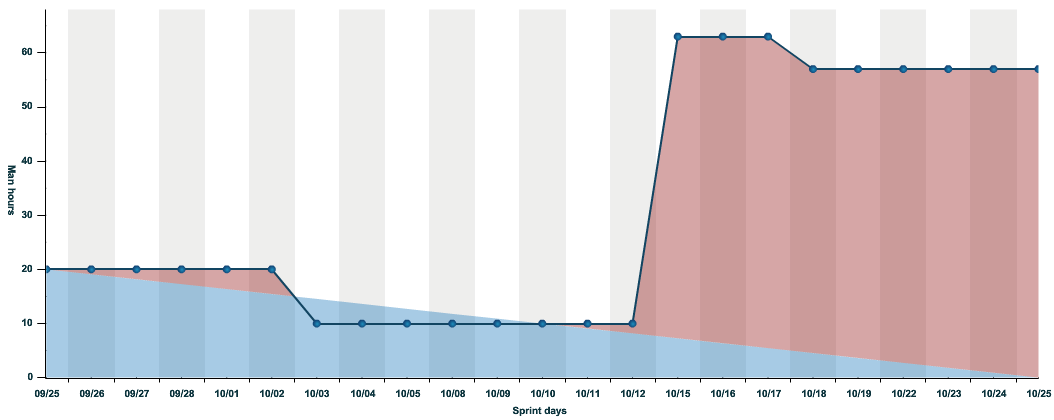
\includegraphics[width=11cm]{burndown-S1.png}
\end{center}
	\caption{Burdown chart du sprint 1}
\end{figure}

L'activité principale de ce premier sprint a été de créer une couche modèle pour notre application. Ceci impliquait de trouver une bibliothèque permettant de lire le format dicom et qui soit compatible avec android. Cette tache a demandé beaucoup d'investissement et de recherche et n'a pu être achevée qu'au sprint suivant. C'est pourquoi on remarque trois plateaux de stagnation. L'augmentation spectaculaire du nombre d'homme-heure restant vers la fin du sprint est du à une mauvaise utilisation de l'outil. En effet, ce sprint nous a introduit à la méthode \emph{scrum} et aux outils associés. De ce fait, notre manque d'assurance et de maîtrise explique les imperfections de ce sprint. Néanmoins, on constate tout de même que des avancées significatives ont pu être réalisées durant ce sprint, la partie modèle étant en majorité achevée lors du passage au deuxième sprint.

\subsubsection{Sprint 2}

\begin{figure}[h]
\begin{center}
	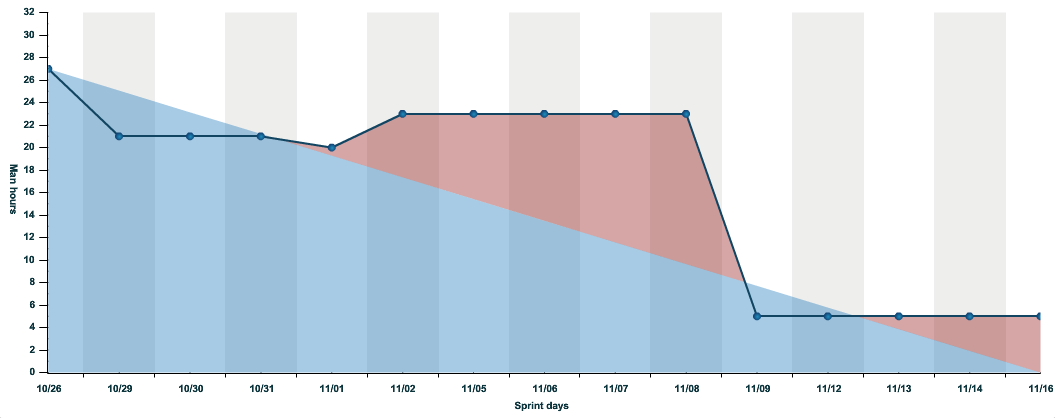
\includegraphics[width=11cm]{burndown-S2.png}
\end{center}
	\caption{Burndown chart du sprint 2}
\end{figure}

Après la prise en main de la méthode \emph{scrum} et des outils au cours du premier sprint, nous avons pu aborder ce deuxième sprint plus en confiance. On constate un bon départ, les tâches les plus faciles ayant été réalisées en premier. Des tâches plus ardues ont ralenti la progression vers le milieu du sprint, mais nous avons su travailler de concert pour surmonter les difficultés et revenir en deçà de la prévision. Les quelques tâches inachevées ont été reportées au dernier sprint. Globalement, ce deuxième sprint est très positif, notre première expérience en \emph{scrum} nous permettant de mieux gérer l'évaluation et la répartition des tâches. Le seul point négatif est la présence de tâches inachevées, c'est pourquoi nous avons décider de revoir notre capacité de travail à la baisse pour le sprint final.

\subsubsection{Sprint 3}

\begin{figure}[h]
\begin{center}
	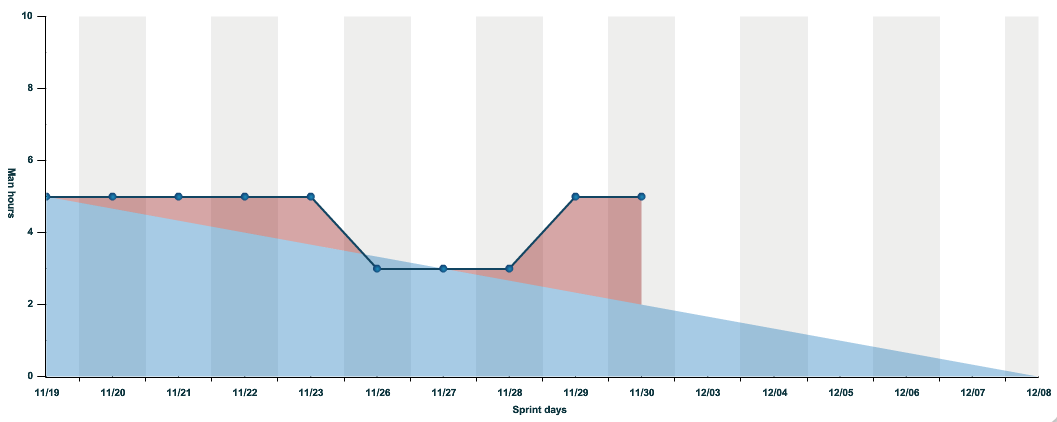
\includegraphics[width=11cm]{burndown-S3.png}
\end{center}
	\caption{Burndown chart du sprint 3}
\end{figure}

Les quelques difficultés rencontrées en début de sprint 3 ont pu être surmontées grâce au concours de toute l'équipe. Les tâches restantes en fin de sprint 2 et les tâches simples du sprint 3 ont été rapidement réalisées. On peut remarquer une augmentation du travail à réaliser. Ceci est du à la modification d'un besoin par le client et son intégration au sprint. Malheureusement, ce sprint n'a pas pu être mené à son terme à cause des impératifs calendaires de rendu.
%partie à modifier en fonction de l'issue du BMI3D
